\documentclass[11pt]{article}
\usepackage[margin=1in]{geometry}
\usepackage{amsmath,amssymb}
\usepackage{graphicx}
\usepackage{booktabs}
\usepackage[hidelinks]{hyperref}
\usepackage{microtype}

\title{Quantized Small Judges: A Preregistered Deployment-Precision Study\\ of a Production Verification Judge}
\author{Chunxiao Wang\\
        nautilus-compass, Nautilus Platform\\
        \texttt{chunxiaoxx@gmail.com}}
\date{October 2026}

\begin{document}
\maketitle

\begin{abstract}
Small language models are increasingly deployed as verification judges, yet their
robustness to post-training quantization --- the default cost-saving step in
production --- remains unstudied. We present a preregistered deployment-precision
study of a production three-state verification judge (Qwen3-1.7B + LoRA adapter,
88.5\% binary accuracy, ECE 0.072), evaluating four precision configurations
$\times$ two decoding regimes over 291 held-out cases. Under a preregistered
agreement gate ($\geq$99\% label agreement with the bf16 anchor), fp16 passes with
\textbf{zero label drift} (1.0000), while int8 (0.9828, five flips) and int4-nf4
(0.9416, seventeen flips) fail the gate. Drift increases monotonically with
quantization strength, corroborating an independent 3B-scale observation. We
release the full per-case judgment matrix, the frozen gating criteria, and a
four-rule deployment discipline for verification judges, and discuss implications
for registry-based self-improving judge systems where a drifting judge silently
corrupts the training signal of the entire loop.
\end{abstract}

\section{Introduction}
Verification judges --- small models that grade the outputs of other models ---
are becoming infrastructure: LLM-as-judge pipelines, agent-harness evaluation
services, and self-improving training loops all depend on them. Quantization is
the default cost-saving step when serving such judges in production, yet the
effect of post-training quantization on \emph{judgment stability} has, to our
knowledge, not been studied; a recent survey of small-language-model judges
likewise notes that their robustness is under-examined.

Our perspective is narrower than ``do quantized models get worse'': a judge in a
registry-based self-improving loop is not a one-off evaluator but \textbf{the
source of training signal} --- every mis-flip it produces becomes (incorrect)
training data. Quantization drift in such a judge does not merely distort one
leaderboard; it silently corrupts the loop itself. This motivates treating
judgment agreement, not task accuracy, as the primary metric.

We contribute: (1) the first preregistered deployment-precision verdict for a
production judge, with a frozen agreement gate; (2) a four-rule deployment
discipline (bf16/fp16 only for production judges, criteria-freeze, U-state
honesty, two-way judging records); (3) a reproducible methodology with all
per-case artifacts released.

\section{Setup}
\begin{itemize}
  \item \textbf{Judge}: NACRE judge instance v1 --- Qwen3-1.7B + LoRA (r16/$\alpha$32,
        adapter sha16 dbcbab6f\ldots), three-state verdicts (pass / fail /
        insufficient\_evidence), production accuracy 88.5\% (ECE 0.072).
  \item \textbf{Data}: 291 held-out cases, disjoint from train/dev by qid
        (leakage-guarded); prompts from the training template family with the
        judge-output channel removed (no oracle leakage).
  \item \textbf{Configurations}: \{bf16, fp16, int8-bnb, int4-nf4\} $\times$
        \{greedy, $T{=}0.3$\}; all runs on merged weights (bypassing the
        peft$\times$bnb hook so the adapter is quantized with the base model,
        matching production serving).
  \item \textbf{Preregistered gate}: a precision is deployable iff greedy label
        agreement with bf16-greedy is $\geq$99\% on the frozen set (tolerance
        $\leq$2/291 flips).
\end{itemize}

\section{Results}

\begin{table}[h]
\centering
\begin{tabular}{lllll}
\toprule
Config & Three-state acc & Agreement vs bf16 & Gate ($\geq$99\%) & Verdict \\
\midrule
bf16 (anchor) & 0.8797 & --- & --- & reference \\
fp16 & 0.8797 & \textbf{1.0000} & pass & deployable \\
int8-bnb & 0.8694 & 0.9828 (5 flips) & fail & not for prod \\
int4-nf4 & 0.8694 & 0.9416 (17 flips) & fail & forbidden \\
bf16 + $T{=}0.3$ & --- & 0.9931 & (disclosure only) & keep greedy \\
\bottomrule
\end{tabular}
\caption{Deployment-precision verdicts under the preregistered agreement gate.}
\label{tab:verdicts}
\end{table}

Three observations: (1) drift grows monotonically with quantization strength;
(2) an independent 3B-scale judge showed the same direction (0.8173 at 4-bit),
suggesting a systematic property rather than a model-specific artifact;
(3) \textbf{agreement must be measured on parsed labels, not raw output
equality} --- a verbatim-equality metric produces all-fail results for any
quantized model and would have invalidated the study had we not caught it
during script review.

\begin{figure}[h]
\centering
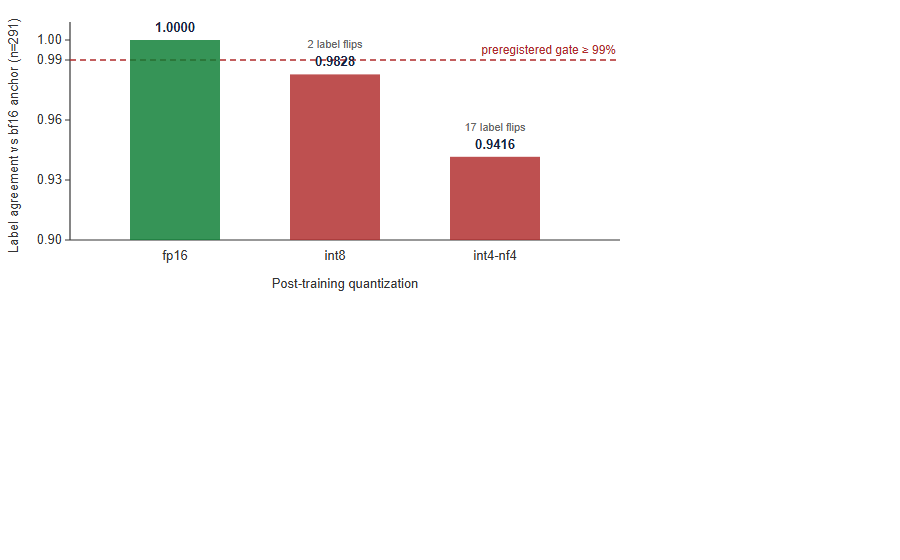
\includegraphics[width=0.8\linewidth]{precor_fig1.png}
\caption{Label agreement vs.\ quantization strength.}
\label{fig:agreement}
\end{figure}

\section{A Deployment-Precision Discipline for Verification Judges}
From these results we distill four rules, all enforced in our production
deployment:
\begin{enumerate}
  \item \textbf{Precision gate.} A judge may serve in production at a given
        precision iff greedy label agreement with the bf16 anchor is $\geq$99\%
        on a frozen held-out set (preregistered; may only be tightened). For our
        judge: fp16 yes; int8 and int4 no.
  \item \textbf{Criteria freeze.} The gate, the held-out set, and the prompt
        template are sha-anchored before any deployment change; loosening
        requires re-registration.
  \item \textbf{U-state honesty.} When the judge cannot decide, it must emit
        insufficient\_evidence rather than guess; deployment changes may not
        trade U-rate for accuracy.
  \item \textbf{Two-way judging records.} Judges err too; every correction feeds
        an errata channel that retrains the judge --- which is precisely why
        rule~1 must hold for every redeployment, or the errata loop amplifies
        noise instead of removing it.
\end{enumerate}

Interaction with registries: judge drift is a systematic noise source in
precedent registries; periodic re-anchoring on held-out sets (our L0--L3 anchor
chain) bounds the drift.

\section{Related Work}
Each neighboring thread examines one face of the problem; none crosses them.
A survey of small-language-model judges~\cite{slmsurvey} flags robustness as
under-studied but does not test quantization. A preregistered study of
post-training quantization~\cite{ptqwelfare} (2026) examines welfare-relevant
behaviors of general models, not judges. Rubric-preference-drift attacks
(RIPD)~\cite{ripd} show natural-language rubrics can be manipulated --- a
concern orthogonal to precision, and one our criteria-freeze rule partially
addresses. Harness-efficiency benchmarks such as Claw-SWE-Bench~\cite{clawswebench}
measure how well agents perform under evaluation but not whether the evaluator
itself survives deployment changes. Our study sits in the unoccupied
intersection: quantization $\times$ small judges $\times$ deployment gating,
with the loop-corruption motivation unique to registry-based systems.

\begin{thebibliography}{9}
\bibitem{slmsurvey} \emph{Small Language Models as Judges: A Survey}. OpenReview, 2026. (60+ works, SLMs $\leq$14B; robustness noted as under-examined.)
\bibitem{ptqwelfare} \emph{Does post-training quantization change welfare-relevant indicators?} --- A preregistered study. LessWrong, 2026-08-10.
\bibitem{ripd} \emph{Rubrics as an Attack Surface: Stealthy Preference Drift (RIPD)}, as catalogued in the promptfoo LLM Security Database.
\bibitem{clawswebench} \emph{Claw-SWE-Bench: A Benchmark for Evaluating Coding Agent Harnesses}. arXiv:2606.12344, 2026.
\end{thebibliography}

\section{Limitations \& Negative Results}
Single judge instance: generalization to other judges is claimed only as
direction, not established. Soft-dimension (confidence-tier) agreement data was
lost to an engineering defect in this round (non-incremental CSV write); the
rerun is registered and pending. Per-case flip lists are summarized as aggregate
agreement here; the full matrix is released in the artifact bundle. We also
report a negative methodological result prominently rather than in a footnote:
our first review of a collaborator's replay script revealed a verbatim-equality
metric that would have produced all-fail results for every quantized
configuration --- caught only because we re-derived the expected agreement by
hand before running.

\section{Artifacts}
All released and sha-anchored: the frozen criteria document, the
merge-then-quantize runner, the per-case judgment matrix, and run logs, in the
nautilus-compass repository (\url{https://github.com/chunxiaoxx/nautilus-compass})
and the nautilus-compass Hugging Face organization
(\url{https://huggingface.co/nautilus-compass}). The judge model card
(nacre-judge-v1, adapter sha16 dbcbab6fd1ff5821) carries the
deployment-precision table on its face.

\end{document}
